\documentclass{article}
\usepackage{graphicx}

\title{ASTR 575 Midterm}
\author{Laurel Farris}
\date{21 October 2015}

\begin{document}
\maketitle

\section{Summary}

For the previous question, I calculated the integral of a function both 
analytically and numerically using Simpson's Algorithm. I also attempted to 
improve the accuracy by dividing the integral into smaller and smaller 
pieces and summing them up. The standard deviation between the results from 
this method and the analytical result are plotted in figure \ref{accuracy}, 
but clearly, something went wrong.

\begin{figure}[h]
  \centering
  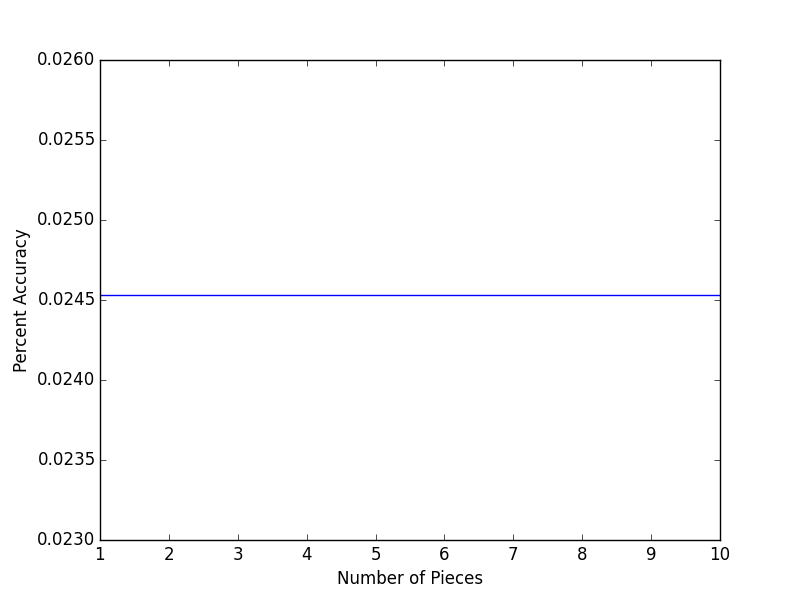
\includegraphics[width=5.0in]{../q3/figure_1.png}
  \caption{This is the plot from q3, part f.}
  \label{accuracy}
\end{figure}

\end{document}
